\chapter{Metodologia}

\section{SVM para Regressão}
A Máquina de Vetores de Suporte (SVM - \textit{Support Vector Machine})
é uma técnica que pode ser aplicada tanto em problemas de classificação quanto de
regressão. A diferença entre os dois casos é que, na regressão, os vetores e as
margens não são usados para separar os dados em classes, mas sim são traçados com o 
objetivo de encontrar uma reta que descreve o comportamento dos dados. As margens
continuam tendo o papel de minimizar os erros \cite{noronha2016implementaccao}. A Figura 
\ref{fig:SVM_1}, mostra graficamente como os vetores são traçados com objetivo achar um padrão 
entre os dados. 

\begin{figure}[h]
  \centering
  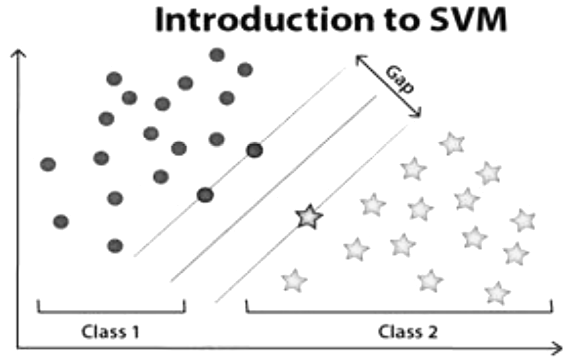
\includegraphics[width=8cm]{figuras/SVM/SVM_1.png}
  \caption{Regressão por SVM, Figura de \cite{Coutinho_2020}.}
  \label{fig:SVM_1}
\end{figure}

\section{Regressão Linear Simples}

A Regressão Liner Simples é um método estatístico que permite estimar a relação entre
duas variáveis, como mostra a Equação \ref{eq:simple}: uma variável explicativa x e uma
variável resposta y, com relação aos coeficientes exitem diversas formas de calcula-los,
técnicas mais comuns são as baseadas em mínimos quadrados ordinários e gradiente descendente
\cite{Almeida_Carvalho_Menino}.

\begin{equation}
  y_{i} = \alpha + \beta x_{i}
  \label{eq:simple}
\end{equation}

\begin{itemize}
  \item $y_{i}$: Variável resposta ou alvo;
  \item $x_{i}$: Variável explicativa;
  \item $\alpha$: Coeficiente de intercepto;
  \item $\beta$: Coeficiente angular.
\end{itemize}

\section{Regressão Linear Múltipla}
A Regressão Linear Múltipla é semelhante à técnica mencionada anteriormente, com a única distinção de
que envolve mais de uma variável explicativa, como indicado na Equação \ref{eq:multi} \cite{Almeida_Carvalho_Menino}.

\begin{equation}
  y_{i} = \alpha + \beta x_{i1} + \beta x_{i2} + \beta x_{i3} + ... + \beta x_{in}
  \label{eq:multi}
\end{equation}